\chapter{INTRODUCTION}
% what is vSLAM
\acrlong{slam} (\acrshort{slam}) is the process of concurrent construction of environmental model and ego-motion of an agent, such as a vehicle, robot, or human, with on-board sensor(s). 
As a major branch of the community, \acrlong{vslam} (\acrshort{vslam}) restricts itself to use visual sensors, e.g. cameras, as the only source of external information. 
\acrshort{vslam} algorithms have been extensively proposed in the field of computer vision and robotics due to the compact sensor configuration and the consequent broader range of application scenarios, e.g. AR/VR, wearable computing, and drone navigation. 

% challenging outdoor vSLAM
By far, \acrshort{vslam} community has made astonishing progress over the past 20 years, establishing {\em de-facto} standard paradigms and enabling various real-world applications.
The successful demonstrations have been frequently reported in the field of indoor robotic navigation and outdoor autonomous driving.
However, the development of \acrshort{vslam} systems has been heavily relying on a few popular benchmarks, e.g. KITTI, that cover limited scenarios, working environments, and favorable lighting conditions compared to real-life cases. 
Towards a robust \acrshort{vslam} system design, the various challenges including moving objects, changing lighting, various weather conditions, and even cross-seasonal appearance changes need to be handled explicitly or implicitly to avoid failures. 
Unfortunately, most state-of-the-art approaches fail to deliver under such inconsistencies, which is especially true for life-long outdoor autonomy. 
The main purpose of this thesis is to push the limits of existing \acrshort{vslam} algorithms, making it possible to deal with a wider type of uncertainties in real-world settings. 

% Overview of section
In this chapter, we review the general pipeline of \acrshort{vslam} paradigms and discuss the major restrictions that prevent their usage on life-long outdoor robotic applications. Afterward, the contributions to alleviate the mentioned limitations are listed and briefly outlined. 

\section{Antonomy of Modern vSLAM System}
\label{sec:intro_slampipeline}

\begin{figure}[t]
    \centering
	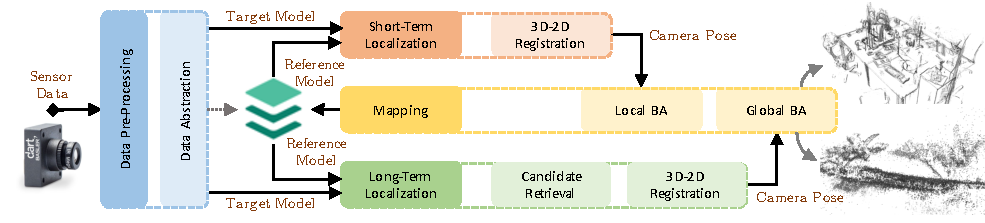
\includegraphics[width=1.0\textwidth]{figures/intro/slam.pdf}
	\caption[Antonomy of Modern \acrshort{vslam} System]{\textbf{Antonomy of Modern \acrshort{vslam} System.} Typically, {\em front-end} consists of data pre-processing, short- and long-term localization, while {\em back-end} refers to mapping layer that performs \acrlong{map} (\acrshort{map}) based dual estimation.
	\label{fig:intro_slampipeline}}
\end{figure}

% General architecture of vSLAM
The architecture of a \acrshort{vslam} system in \ref{fig:intro_slampipeline} is mainly composed of data pre-processing, short- and long-term localization, and mapping modules. 
In general, the data pre-processing module abstracts the raw images captured from the camera(s) into models that are amenable to camera pose inference. 
Afterward, short- and long-term localization modules register the processed model w.r.t. the selected portion(s) of the reconstructed map.
The reference map portion(s) can either be set as the latest created map for short-term localization or come from a candidate retrieval algorithm, e.g. loop closure detection or image retrieval, for long-term localization. 
Parallelly, the mapping layer jointly optimizes the camera poses and scene structure at a local and/or global scale with the short- and long-term localization inputs as initial conditions. 
This dual estimation is often formulated as a \acrshort{map} problem, which is also known as \acrlong{ba} (\acrshort{ba}) in the field of \acrlong{sfm} (\acrshort{sfm}).

% Front-end and Back-end
Typically, the mentioned components can be categorized into two groups: {\em front-end} and {\em back-end}. 
Data pre-processing, short- and long-term localization can be considered as principal components of \acrshort{vslam} {\em front-end}, while the mapping serves as \acrshort{vslam} {\em back-end}.
Note that one of the major tasks of \acrshort{vslam} is to maintain a locally or even globally consistent map and camera trajectory, which inherently requires {\em back-end} to involve as much camera frames and landmarks as possible.  
To facilitate real-time computation, modern \acrshort{vslam} only passes down-sampled essential camera frames, namely keyframes, and corresponding landmarks into {\em back-end} for acceleration.
Meanwhile, {\em front-end} takes place on regular frames to incrementally estimate current camera pose as initialization for {\em back-end} to compensate for the potentially increased non-convexity of the optimization problem.
As a result, vSLAM {\em front-end} usually operates at a higher frame-rate than {\em back-end}, which works together for accurate and robust estimation within a real-time budget. 

% VO v.s. vSLAM
Another closely related terminology is \acrlong{vo} (\acrshort{vo}), which is named for its similarity to wheel odometry.
\acrshort{vo} incrementally estimates camera motions and locally consistent maps using short-term localization and local \acrshort{ba}. 
Unfortunately, the small errors from the estimation are accumulated over time and finally drift away from their actual positions. 
If a \acrshort{vo} system incorporates modules to detect revisited scenes and perform global optimization, the drift can be eliminated.
From this perspective, \acrshort{vo} can be considered as a reduced \acrshort{vslam} system by omitting the long-term localization and global \acrshort{ba} components.


\section{Toward the Robustness of vSLAM system}
\label{sec:intro_robustness}
% Indirect and Direct
In general, \acrshort{vslam} systems can be categorized into indirect or direct methodology, where each method provides different levels of robustness against sensor and process noise.

\subsection{Robustness of Indirect and Direct Paradigms}
Indirect {\em front-end} pre-processes acquired images to detect and extract a particular type of 2D sparse features, associate and register them w.r.t. a selected portion of reconstructed 3D maps.
Receiving the initialized camera poses, scene structure, and data association, indirect {\em back-end} further refines them through reprojection error minimization.
A good feature usually shows considerable repeatability and discriminability under photometric disturbance and view-point changes.
It guarantees high inlier/outlier ratios during feature matching, which further enables efficient \acrshort{ransac}-based outlier removal and finally delivers accurate state estimation. 
The state-of-the-art features, e.g. ORB and SIFT, have demonstrated to show up such excellent properties and thus make the indirect approaches dominating the research field for years. 
However, the robustness comes with the price of additional computational overhead, which limits the amount of data usage. 
The sparser 3D map, in turn, makes the system fragile at feature-less or feature-ambiguous scenes, e.g. pure natural scenes due to perceptual aliasing, where not enough good features can be extracted and successfully tracked. 


Direct {\em front-end} utilizes raw data of the image to estimate camera motions and surrounding environment based on the Lucas-Kanade by making brightness constancy assumption. 
Similarly, the direct {\em back-end} jointly optimize camera poses and environmental model through photometric error minimization without explicit data associations. 
Decoupled with certain types of features, direct pipelines end up with higher flexibility of image information usage compared to the indirect ones. 
Without computationally intensive feature extraction and matching process, the direct approach allows for denser 3D map maintained in real-time, which makes it possible to operate in challenging feature-less environments.
However, the brightness constancy assumption makes the direct alignment approach very sensitive to unmodeled photometric disturbance, e.g. camera auto-exposure and environmental lighting changes.
Worse still, the direct image alignment suffers from the small region of attraction due to the non-smoothness nature of the image.
Although the image-pyramid-based coarse-to-fine direct alignment strategy has proven to alleviates the non-convexity of the problem, the accuracy of the direct approach is tightly-dependent on the accuracy of camera pose initialization.
  

\subsection{Gaps of Applicability in State-of-the-Arts}
% module-wise evaluation
To better understand how the above-mentioned limitations affect real-world \acrshort{vslam} systems, we summarize the modular information of the representative \acrshort{vslam} systems in \ref{tbl:intro_gaps} and evaluate their module-wise performance regarding the estimation accuracy in \ref{fig:intro_gaps}. 
The indirect methods, e.g. \textbf{IP} and \textbf{L}, shows superior camera tracking accuracy at all three tests over direct counterparts in structured urban scenes but deteriorate significantly in natural environments.  
In opposite, the direct point (\textbf{DP}) method can always provide moderate short-term localization and local mapping estimation in both urban and natural scenarios. 
However, it fails to deliver similar accuracy at long-term localization where the brightness constancy assumption is violated.  
Interestingly enough, the edge (\textbf{E}) method provides impressive robustness at both short- and long-term localization in the challenging unstructured natural scenes but presents disaster results after \acrshort{ba} optimization. 
Such an issue is suspected to be one of the major reasons \textbf{E} method has only been integrated into RGB-D \acrshort{vslam} systems but monocular ones, which further prevents its usage in outdoor applications.
 
\begin{table}[t]
	\centering
	\caption[State-of-the-Art \acrshort{vslam}/\acrshort{vo} Systems]{\textbf{State-of-the-Art \acrshort{vslam}/\acrshort{vo} Systems.} Basic information of State-of-the-Art \acrshort{vslam}/\acrshort{vo} systems
	\label{tbl:intro_gaps}}
	\resizebox{1.0\textwidth}{!}{%
	\renewcommand{\arraystretch}{1.2}
	\begin{tabular}{c|cccccc}
\hline
\multirow{3}{*}{Method} & \multicolumn{4}{c}{\textbf{Point}}                             & \multirow{2}{*}{\textbf{Line}} & \multirow{2}{*}{\textbf{Edge}} \\
                        & Indirect & Direct   & \multicolumn{2}{c}{Semi-Direct} &                       &                       \\
                        & {\em ORBSLAM}  & {\em DSO}      & {\em SVO}            & {\em LDSO}           & {\em PL-SLAM}               & {\em RE-SLAM}               \\ \hline
Short-Term Localization        & IP        & DP        & DP              & DP              & L+IP                   & E                     \\
Mapping                & IP        & DP        & IP              & DP              & L+IP                   & E                     \\
Long-Term Localization               & IP        & -         & -               & IP              & IP                     & E                     \\ \hline
Sensor Setup            & M/S/RGBD & M/S/RGBD & M/S/RGBD       & M/S/RGBD       & M/S/RGBD              & RGBD                  \\
Environment             & IN/OUT   & IN/OUT   & IN/OUT         & IN/OUT         & IN                    & IN                    \\ \hline
	\end{tabular}
	\renewcommand{\arraystretch}{1}
}
{\footnotesize * IP - Indirect Point, DP - Direct Point, L - Line, E - Edge, M - Mono Camera, S - Stereo Rig, RGBD - RGBD Camera, IN - Indoor, OUT - Outdoor}
\end{table}

\begin{figure}[t]
    \centering
	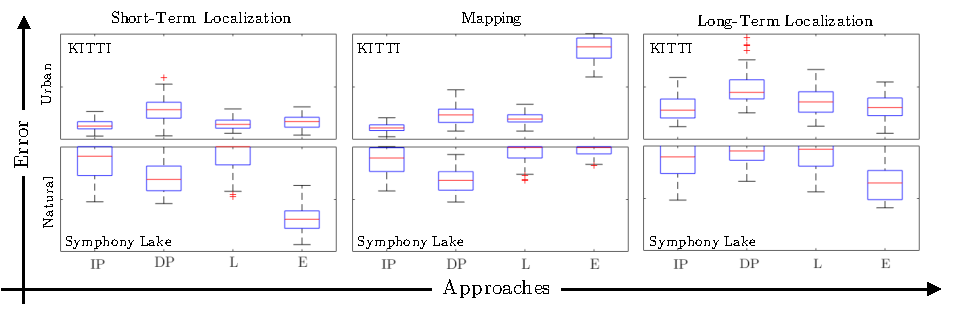
\includegraphics[width=1.0\textwidth]{figures/intro/compareMethods.pdf}
	\caption[Module-wise Evaluation of State-of-the-Art \acrshort{vslam} Paradigms]{\textbf{Module-wise Evaluation of State-of-the-Art \acrshort{vslam} Paradigms.} \textbf{Top-Row}: Evaluation in structured urban scenes. \textbf{Bottom-Row}: Evaluation in unstructured natural scenes. \textbf{Left-Column}: Evaluation on short-term localiztion. \textbf{Mid-Column}: Evaluation on mapping. \textbf{Right-Column}: Evaluation on long-term localiztion.
	\label{fig:intro_gaps}}
\end{figure}


% short-term failure mode
To understand the rationale behind the performance degeneration, we propose to analyze the failure modes of indirect and direct paradigms in \ref{fig:intro_vofailures}. 
When the environment is well structured, the indirect method shows considerable robustness against non-smooth camera motions compared with the direct methods. 
Such observation coincides with the previous analysis that the direct methods generally presents a much smaller region of attraction due to the non-smooth nature of the image, which shrinks their convergence basin during optimization. 
However, when it comes to natural environments, the rapidly growing incorrect data association easily dominates the indirect pose initialization and joint optimization, making the system more fragile than others.  
By contrast, the direct method can always preserve enough but less accurate pixel correspondences through direct image alignment, making it a more favorable scenario for unstructured environments. 
As the expense, it is more sensitive to lighting changes, e.g. over-exposures and lens flares, which limits its life-long operation.

\begin{figure}[t]
    \centering
	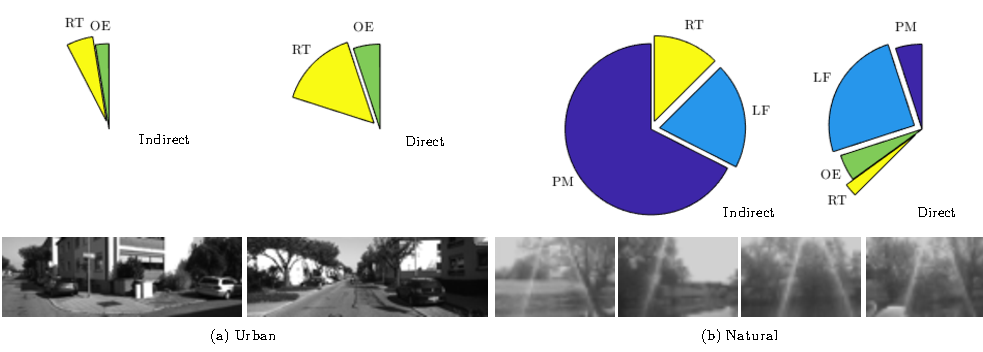
\includegraphics[width=1.0\textwidth]{figures/intro/vofailures.pdf}
	\caption[Typical Failure Modes of Short-Term Localization]{\textbf{Typical Failure Modes of Short-Term Localization.} Typical failure modes in urban (\textbf{Left}) and natural (\textbf{Right}) scenes. LF - Lens Flare, PM - Poor Matches, RT - Rough Turn, OE - Other Effects
	\label{fig:intro_vofailures}}
\end{figure}

% Issues of long-term operation
Although problematic, short-term robustness issue connected to incorrect data association or brightness constancy assumption is usually considered as the easier one to tackle.
The long-term localization between day and night or different seasons is a significantly more challenging problem due to the large perception changes in the acquired images as shown in \ref{fig:intro_locfailures}. 
In recent years, the appearance-based approaches have demonstrated their superior performance on image-level retrieval, but the long-term localization in \acrshort{vslam} pipeline is topological in nature.
Current model representations still lack sufficient repeatability and discriminability to work reliably under such circumstances.  

\begin{figure}[t]
    \centering
	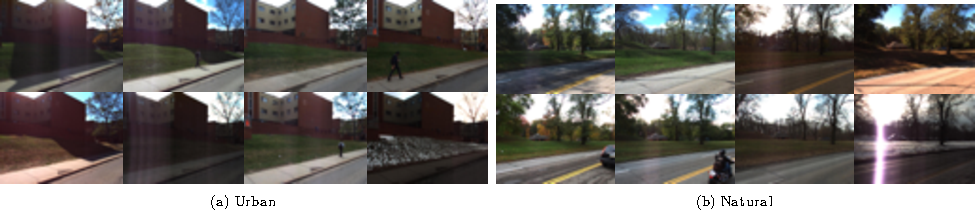
\includegraphics[width=1.0\textwidth]{figures/intro/locfailures.pdf}
	\caption[Challenging Scenarios for Long-Term Localization]{\textbf{Challenging Scenarios for Long-Term Localization.} Localization across seasons in urban (\textbf{Left}) and natural (\textbf{Right}) scenes.
	\label{fig:intro_locfailures}}
\end{figure}

% Summary
In summary, the robustness of state-of-the-art \acrshort{vslam} short-term operations is tightly-related to the quality of features (indirect) in the environments or illumination conditions (direct) during operation. 
In addition, the problem can escalate when it comes to life-long operation, where the camera localization across large perception changes comes to end. 

\section{Robotic Applications}
\label{sec:intro_applications}

\begin{figure}[t]
    \centering
	\includegraphics[width=1.0\textwidth]{figures/intro/roboticapp.pdf}
	\caption[Robotic Applications of \acrshort{vslam}]{\textbf{Robotic Applications of \acrshort{vslam}.} Three typical robotic appliations in need of robotic \acrshort{vslam} systems: agriculture robotics (\textbf{Top-Left}), environmental monitoring (\textbf{Top-Right}), and autonomous driving Agriculture robotics (\textbf{Bottom})
	\label{fig:intro_roboticapp}}
\end{figure}

% Agricultural robotics
One of the research fields that favors robust \acrshort{vslam}/\acrshort{vo} originated from the rapid development of precision agriculture. 
For agriculture robotics, the wheel odometry is suspected of being insufficient due to uneven ground surface and slippery terrain conditions. 
To obtain the wheel slippage invariance, the \acrlong{gps} (\acrshort{gps}) and \acrlong{imu} (\acrshort{imu}) systems are typically fused to deliver the motion estimates, therefore helping to achieve high-precision navigation and in-field actuation. 
However, the investment to build a high-end perception system to deliver the millimeter-level localization is usually unacceptable for small research groups or companies due to the exceptionally high price of accurate sensors, such as high-performance \acrshort{imu} or real-time kinematic \acrshort{gps}. 
In contrast, the cost of a high-end camera has steadily declined in recent years, which promotes \acrshort{vo} solutions as an excellent complement to the expensive \acrshort{gps}/\acrshort{imu} systems.

% Natural Monitoring
High demand for robust \acrshort{vslam}/\acrshort{vo} techniques also appears in the field of robotic environmental assessment and monitoring. 
Even though monitoring the natural environment is a task that is highly application-dependent, most systems require the perception system to hold significant robustness against outdoor disturbances, such as lighting changes and the high complexity of the monitored scenes. 
The well-established methodologies for such tasks use either range sensors, such as 3D LIDAR, 2D range-scanner to formulate point clouds for \acrshort{icp}-based registration. 
However, the high price and energy costs prevent their use for on-board long-term operations. 
In contrast, cameras can serve as a more versatile and compact solution compared with existing methods.
Moreover, the images are inherently more informative than point clouds from laser sensors, hence being more suitable for environmental assessment and monitoring applications.

% Autonomous Driving
As a rapidly advancing area, autonomous driving also shows considerable interest in robust \acrshort{vslam}/\acrshort{vo} techniques.
Compared with robotic applications that require energy- and computation-friendly motion estimation and mapping systems, autonomous driving applications can afford computationally expensive and energy-consuming devices installed onboard. 
Therefore, the industry has put more and more attention to Lidar-based solutions due to their stability and accuracy compared to the pure visual approaches. 
However, the point cloud, as sparse geometric features, is, in essence, less informative than visual cues, which can be problematic when geometric features are absent, e.g. in high-way or tunnel scenes.
As a compensation, visual cues can provide richer information to Lider-based systems, which makes it possible to perform more robust data association for short- and especially long-term operations, e.g. localization across seasons or semantic mapping applications.

\section{Outline of Thesis}
\label{sec:intro_outlineofthesis}
The rest of this thsis is organized as shown in \ref{fig:intro_overview}:

\begin{sidewaysfigure}[t]
    \centering
	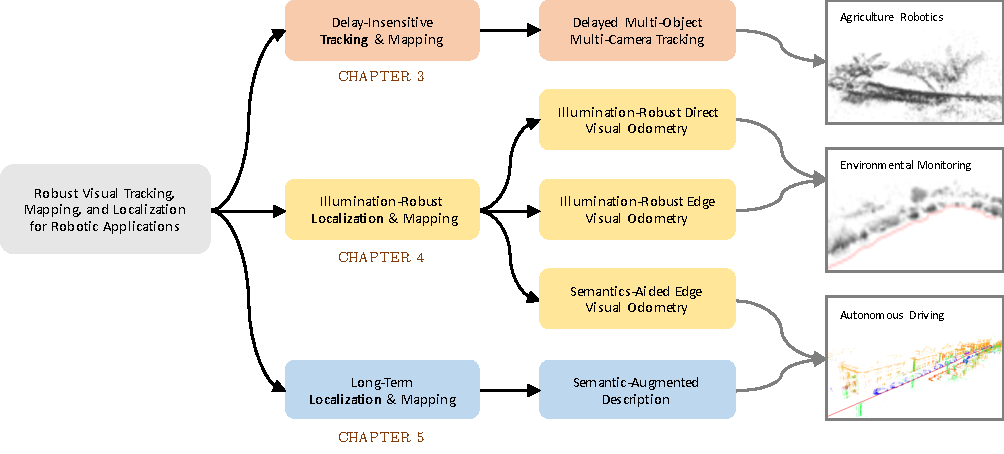
\includegraphics[width=0.8\textwidth]{figures/intro/overview.pdf}
	\caption[Outline of Thesis]{\textbf{Outline of Thesis.}
	\label{fig:intro_overview}}
\end{sidewaysfigure}

\begin{enumerate}
	\item \textbf{Chapter 2} describes the mathematical foundations of the general \acrshort{vslam} problem, from the underlying \acrshort{map} estimation, typical energy functions used in multiple modules, to least-square optimization in Lie-Manifold. The major perspective of this thesis is to extend the applicability of the golden-standard \acrshort{vslam} paradigms for outdoor life-long autonomy. Thereby, understanding the underlying logic and major assumptions behind \acrshort{vslam} estimation problem is of paramount importance.
	\item \textbf{Chapter 3} describes a delay-insensitive multi-object non-overlapping camera tracking system, which aims to provide flexibility for the weed control system in dealing with the indeterminate classification delays. To achieve metric 3D multi-object tracking across camera, a monocular-sonar \acrshort{vo}, an illumination-robust cross-camera object tracking, and a delay-insensitive object management system are deliberately designed to overcome typical challenges in agricultural environments. The proposed object tracking module is implemented and evaluated on a weed control machine in a real-world sugar beet field for automated weed removal. 
	\item \textbf{Chapter 4} describes illumination-robust \acrshort{vo} systems that are capable of dealing with typical lighting changes in outdoor environments, thereby providing reliable camera motion and scene structure estimation for long-term autonomy. First, an illumination-robust direct \acrshort{vo} system is presented, where a convergence-preserved joint optimization strategy is proposed to achieve high-precision motion estimation while preserving a large convergence basin. Later, a monocular edge \acrshort{vo} framework, comprised of \acrshort{icp}-based edge alignment, edge-guided data association, and graph-based local \acrshort{ba}, is proposed to further improve the stability of \acrshort{vslam} system by implementing illumination-robust edge features. Finally, a semantic extension of our proposed edge \acrshort{vo} is described to reconstruct large-scale semantic maps for long-term autonomy. The proposed methods are implemented and evaluated on an automated surface vehicle in pure natural scenes for lakeshore monitoring.
	\item \textbf{Chapter 5} describes a deep neural network, namely {\em DLSSNet}, that simultaneously learns low-level geometric descriptor and high-level semantic segmentation for long-term localization tasks in the context of autonomous driving. We show that the semantic segmentation and local feature description can be simultaneously learnt within the hierarchy of a single deep network pipeline. The augmented multi-level descriptors, trained in an end-to-end manner, provide a more stable high-level representation for local feature dis-ambiguation as compared to other architectures. The proposed methods are implemented and evaluated on an autonomous car in urban scenes for cross-season localization.

\end{enumerate}